% XCircuit output "BlockDiagram.tex" for LaTeX input from BlockDiagram.eps
\def\putbox#1#2#3#4{\makebox[0in][l]{\makebox[#1][l]{}\raisebox{\baselineskip}[0in][0in]{\raisebox{#2}[0in][0in]{\scalebox{#3}{#4}}}}}
\def\rightbox#1{\makebox[0in][r]{#1}}
\def\centbox#1{\makebox[0in]{#1}}
\def\topbox#1{\raisebox{-0.60\baselineskip}[0in][0in]{#1}}
\def\midbox#1{\raisebox{-0.20\baselineskip}[0in][0in]{#1}}
   \scalebox{0.7}{
   \normalsize
   \parbox{8.53125in}{
   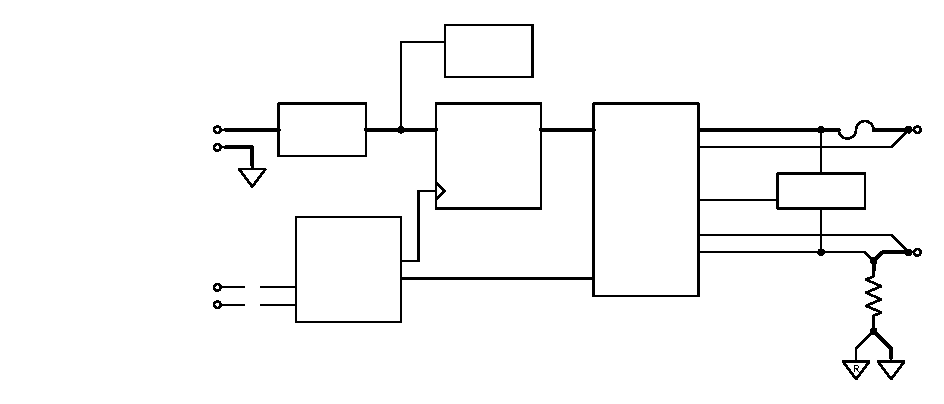
\includegraphics[scale=1.42857]{BlockDiagram}\\
   % translate x=1250 y=282 scale 0.26
   \putbox{2.91in}{2.54in}{1.20}{\centbox{\midbox{Input}}}%
   \putbox{2.91in}{2.37in}{1.20}{\centbox{\midbox{Protection}}}%
   \putbox{4.50in}{3.29in}{1.20}{\centbox{\midbox{Local}}}%
   \putbox{4.50in}{3.12in}{1.20}{\centbox{\midbox{Regulators}}}%
   \putbox{4.50in}{2.20in}{1.20}{\centbox{\midbox{Preregulator}}}%
   \putbox{6.00in}{1.87in}{1.20}{\centbox{\midbox{Regulator}}}%
   \putbox{1.83in}{2.37in}{1.20}{\rightbox{\midbox{\SI{24}{V} \SI{3}{A}}}}%
   \putbox{1.75in}{0.95in}{1.20}{\rightbox{\midbox{Loop In}}}%
   \putbox{1.75in}{0.79in}{1.20}{\rightbox{\midbox{Loop Out}}}%
   \putbox{2.25in}{0.87in}{1.20}{\rotatebox{-270}{\centbox{\midbox{ISOLATION}}}}%
   \putbox{6.58in}{2.54in}{0.84}{\midbox{Regulated power}}%
   \putbox{6.58in}{2.37in}{0.84}{\midbox{Pos. feedback}}%
   \putbox{6.58in}{1.54in}{0.84}{\midbox{Neg. feedback}}%
   \putbox{6.58in}{1.37in}{0.84}{\midbox{Current feedback}}%
   \putbox{7.66in}{1.95in}{1.20}{\centbox{\midbox{Overload}}}%
   \putbox{7.66in}{1.79in}{1.20}{\centbox{\midbox{Protection}}}%
   \putbox{3.16in}{1.45in}{1.20}{\centbox{\midbox{Controller}}}%
   \putbox{3.58in}{1.20in}{0.84}{\rightbox{\midbox{PWM}}}%
   \putbox{3.58in}{1.04in}{0.84}{\rightbox{\midbox{DAC/ADC}}}%
   \putbox{2.75in}{0.87in}{0.84}{\midbox{UART}}%
   } % close 'parbox'
   } % close 'scalebox'
   \vspace{-\baselineskip} % this is not necessary, but looks better
